\subsection{Variational Tree Walk}

\subsubsection{Microbiota dataset}

As we look into the microbiota data, we notice a major phylogenetic architecture to describe various levels of precision in the microbiota composition.
Indeed, such phylogenetic structure can be represented as a tree as on the following figure:
\begin{figure}[H]
    \center
    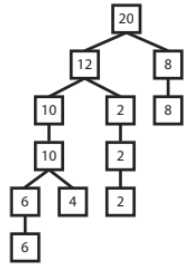
\includegraphics[scale=1]{images/abundance_tree_phylogenetic}
    \caption{Phylogenetic tree example with abundance data (in the nodes) at each layer of the tree.
    Each node represents a bacterium specie at a given precision layer in the tree. From \cite{microbiome_deeplearning_research}.}
    \label{fig:phylogenetic_tree}
\end{figure}

Such structure can not be used directly in a machine learning system since it's not a vectorizable representation.
Hence, we first suggest to transform the tree in a matrix to image structure as in the following example:
\begin{figure}[H]
    \center
    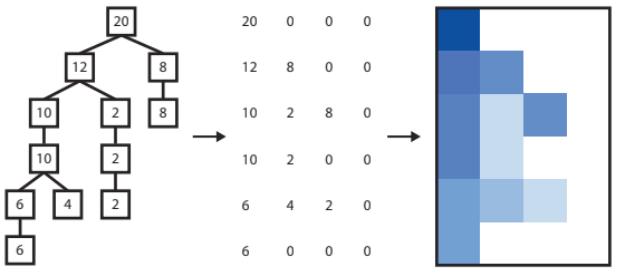
\includegraphics[scale=1]{images/tree_to_image}
    \caption{Phylogenetic tree to image representation:
    opacity of the pixel relates to the abundance of the species at the given level of precision (normalized between 0 and 1).
    From \cite{microbiome_deeplearning_research}.}
    \label{fig:phylogenetic_tree_to_img}
\end{figure}

Sadly this image representation does not convey the link between the species abundance given by the edges of the tree.
As a result, we suggest to find a hidden variable $Z$ that uses the adjacent matrix of the tree $T$, to find a way to go through the image
as for the PixelCNN approach.
Such approach, in addition to use the adjacency of the tree graph, would then learn an interesting trajectory to compute the correlation between the abundance data.
The next section offers the mathematical framework of the proposed idea.

\subsubsection{Framework and optimization objectives}

\subsubsection{EM approach}

In first approximation, we would like to use the EM algorithm to try to compute the following latent model:
\begin{itemize}
    \item We assume that we have $n$ individuals observed through $(X_i, T_i)_{1 \leq i \leq n}$.
    \item The maximum depth of a phylogenetic tree is $D$, the maximum number of nodes $N_{nodes}$, and the maximum amount of unique species at any level is $U$.
    \item $X_i$ is the abundance matrix of the individual $i$ (image of size $N_{nodes} \times U$) , which is observed.
    \item $T_i$ is the adjacent matrix of the phylogenetic tree of individual $i$, of size $N_{nodes} \times N_{nodes}$, which is observed.
          We could use any other encoding of a tree (contour function, depth function, ...).
    \item $Z_i$ is a hidden random walk over the tree $T_i$ (discrete vector, permutation of $(1, \dots, N_{nodes})$).
          For a given random walk process over the tree, we denote by $N_{Z}$ the amount of possible generations ($N_Z \leq N_{nodes}!$).
          Hence, $p_{\gamma}(Z_i = z | T_i)$ is a known distribution defined by the random walk process.
    \item Taking inspiration from the PixelCNN, our model should learn the distribution $p_{\omega}(X_i | Z_i, T_i)$ as a CNN/RNN that is masked following $Z_i$.
          We also assume that conditionally to $Z_i$, this distribution is independent from the adjacent matrix: $p_{\omega}(X_i | Z_i, T_i) = p_{\omega}(X_i | Z_i)$.
\end{itemize}

Recall from the EM context that we aim at maximizing
$$
Q(\widehat{\theta}, \theta) = \mathbb{E}_{p_{\widehat{\theta}(Z|X,T)}}[\log p_{\theta}(X, Z, T) | X,T]
$$
Hence, we start with the \textbf{expectation} step and try to evaluate $p_{\widehat{\theta}(Z|X,T)}$:
$$
\begin{align}
    \log p_{\widehat{\theta}}(Z_i|X_i,T_i) = \tau_{ik} &= \log \frac{p(T_i) p_{\widehat{\theta}}(Z_i | T_i) p_{\widehat{\theta}}(X_i | Z_i, T_i)}{\sum_{j=1}^{N_Z} p(T_i) p_{\widehat{\theta}}(Z_i=z_j | T_i) p_{\widehat{\theta}}(X_i | Z_i=z_j, T_i)} \\
                                &= \log \frac{p_{\widehat{\theta}}(Z_i | T_i) p_{\widehat{\theta}}(X_i | Z_i)}{\sum_{j=1}^{N_Z} p_{\widehat{\theta}}(Z_i=z_j | T_i) p_{\widehat{\theta}}(X_i | Z_i=z_j)}
\end{align}
$$
Even though all terms seems computable and explicit here, the summation over $N_Z$ can be very large depending on the complexity of the random walk process we pick.
As a result, we will propose a variational approach to overcome this issue in the next section. \\

As it is right now, one could easily compute the \textbf{maximization} step for $Q(\widehat{\theta}, \theta)$ over $\theta = (\gamma, \omega)$, as it is now explicit:
$$
Q(\widehat{\theta}, \theta) = \sum_{i=1}^n (\log p(T_i) + \log p_{\gamma}(Z_i | T_i) + \log p_{\omega}(X_i | Z_i)) \tau_{ik}
$$

\subsubsection{Variational approach}

In this second approach, we aim at giving a variational algorithm to compute a lower bound to the true objective.
To that end, since it can not be computed directly, we propose an estimate of $p_{\theta}(Z|X,T) = q_{\Phi}(Z|X,T)$.
Recall then the ELBO explicited in the VAE general framework:
$$
\log p_{\theta}(X) = \underbrace{\mathbb{E}_{q_{\Phi}(Z|X,T)}\left[ \log \frac{p_{\theta}(X,Z,T)}{q_{\Phi}(Z|X,T)} \right]}_{ELBO(\Phi, \theta)} + D_{KL}[q_{\Phi}(Z|X,T) \Vert p_{\theta}(Z|X,T)]
$$
Such ELBO can be rewritten as:
$$
\begin{align}
    ELBO(\Phi, \theta) &= \mathbb{E}_{q_{\Phi}(Z|X,T)}[\log p_{\theta}(X,Z,T)] - \mathbb{E}_{q_{\Phi}(Z|X,T)}[\log q_{\Phi}(Z|X,T)] \\
                        &= \mathbb{E}_{q_{\Phi}(Z|X,T)}[\log p_{\theta}(X|Z,T)] - \mathbb{E}_{q_{\Phi}(Z|X,T)}\left[ \log \frac{q_{\Phi}(Z|X,T)}{p_{\gamma}(Z,T)} \right] \\
                        &= \mathbb{E}_{q_{\Phi}(Z|X,T)}[\log p_{\theta}(X|Z)] - D_{KL}[q_{\Phi}(Z|X,T) \Vert p_{\gamma}(Z|T)] + \log p(T)
\end{align}
$$

Designing the prior $p_{\gamma}(Z_i | T_i)$ is no easy task though, as it is completely free-form.
Indeed, using a too free-form prior will end up in not using the tree structure at all by recreating a completely different markov chain
(if any leap can be made in the tree, then the obtained random walk will not necessarily exploit the tree structure).
If the the prior is too restrictive, we might be over-exploiting the phylogenetic structure and obtain an average walk over the tree that is not relevant to each unique case.
Hence, we try to design a prior that takes into account the tree structure while still having some entropy so any random walk is still possible (with low probability).\\

For notation purposes, we introduce the random variable $\eta_k$ that represents the chosen node index at step $k$ of the random walk.
Whatever prior we decide to pick, it feels as most relevant to pick the seed of the markov chain using a learnable distribution,
so that we have $\eta_{1} \sim p(\pi)$ where $\pi = (\pi_1, \dots, \pi_{N_{nodes}})$ .
We also introduce a norm over the tree $\Vert . \Vert_T$ that will enable us to measure the distance between nodes:
\begin{itemize}
    \item Norm of a given node is given by:
        $$
        \Vert \eta_k \Vert_T = \text{distance to root node of the tree}
        $$
    \item Distance computation is given by:
          $$
            \Vert \eta_k - \eta_j \Vert_T = \left\{
            \begin{array}{ll}
                0 & \mbox{if } i = j \\
                \text{number of edges between node $k$ and $j$} & \mbox{otherwise}
            \end{array}
            \right.
          $$
\end{itemize}

The first prior that we propose is a variation of the dirichlet prior, parameterized by $\lambda = (\lambda_1, \dots, \lambda_{N_{nodes}})$.
If we denote by $u_k$ a given node indexed by $k$, let $\alpha_j = (\Vert u_k - \eta_j \Vert_T)_{1 \leq k \leq N_{nodes}}$:
$$
\begin{align}
    d_{k+1} | \eta_{k} &\sim \mathcal{D}(\lambda \odot \alpha_k) \\
    \eta_{k+1} &\sim p(d_{k+1})
\end{align}
$$
Hence, computing $Z_i | T_i$ is given by $Z_i = (\eta_k)_{k \in \{1, \dots, N_{nodes}\}}$ following the previously introduced process:
\begin{algorithm}[H]
    \caption{Tree random walk without replacement}
    \begin{algorithmic}
        \REQUIRE $T_i$ a given tree, $(\pi, \lambda)$ distribution parameters
        \STATE Draw $\eta_{1} \sim p(\pi)$
        \STATE Define $Z_i = (\eta_{1})$
        \For{ $k \in \{2, \dots, N_{nodes}\}$ }
            \STATE \quad Draw a distribution $d_{k} | \eta_{k-1} \sim \mathcal{D}(\lambda \odot \alpha_{k-1})$
            \STATE \quad Mask in $d_{k}$ the already seen nodes in $Z_i$ to obtain $\tilde{d}_{k}$
            \STATE \quad Draw $\eta_{k} \sim p(\tilde{d}_{k})$
            \STATE \quad Update $Z_i = (Z_i, \eta_k)$
        \EndFor:
    \end{algorithmic}

    \textbf{Output:} $Z_i = (\eta_1, \dots, \eta_{N_{nodes}})$

    \label{alg:tree_walk_no_replacement}
\end{algorithm}

Computing $q_{\Phi}(Z_i | X_i, T_i)$ is rather simple at this stage, and it has an explicit formula:
$$
q_{\Phi}(Z_i = (z_1, \dots, z_{N_{nodes}}) | X_i, T_i) = p_{\pi}(z_1) p_{\tilde{d}_1}(z_2) \dots p_{\tilde{d}_{N_{dots}}}(z_{N_{dots}})
$$

Taking inspiration from the VQ-VAE architecture, one might modify the previous algorithm as simple prior sampling denoted by $Z_i^e(T_i)$,
and then a quantization step by taking the $arg\max$ over the output probabilities sampled:
$$
\begin{align}
    d_{k+1} | \eta_{k} &\sim \mathcal{D}(\lambda \odot \alpha_k) \\
    \eta_{k+1} &= arg\max_{j} [d_{k+1}]_j
\end{align}
$$

\begin{algorithm}[H]
    \caption{Tree quantized random walk}
    \begin{algorithmic}
        \REQUIRE $T_i$ a given tree, $(\pi, \lambda)$ distribution parameters
        \STATE Draw $\eta_{1} \sim p(\pi)$
        \STATE Define $Z_i^q = (\eta_{1})$
        \For{ $k \in \{2, \dots, N_{nodes}\}$ }
            \STATE \quad Draw a distribution $d_{k} | \eta_{k-1} \sim \mathcal{D}(\lambda \odot \alpha_{k-1})$
            \STATE \quad Mask in $d_{k}$ the already seen nodes in $Z_i^q$ to obtain $\tilde{d}_{k}$
            \STATE \quad Set $\eta_{k} = arg\max_{j} [\tilde{d}_{k}]_j$
            \STATE \quad Update $Z_i^q = (Z_i^q, \eta_k)$
        \EndFor:
    \end{algorithmic}

    \textbf{Output:} $Z_i^q = (\eta_1, \dots, \eta_{N_{nodes}})$

    \label{alg:tree_quantized_walk}
\end{algorithm}

Sadly, $q_{\Phi}(Z_i|X_i,T_i) \neq \delta_{\{Z_i = Z_i^q\}}$, so we do not fall back on that objective yet:
$$
\begin{align}
    ELBO(\Phi, \theta) &= \sum_{i=1}^n \log p_{\omega}(X_i | Z_i^q(T_i)) - \log \frac{q_{\Phi}(Z_i^q(T_i) | X_i)}{p_{\gamma}(Z_i^q (T_i) | T_i)} \\
    &= \sum_{i=1}^n \log p_{\omega}(X_i | Z_i^q(T_i)) + \log p_{\gamma}(Z_i^q (T_i) | T_i)
\end{align}
$$

Being a random process, the density of a moving random process is yet to be defined.